\documentclass{article}
\usepackage{placeins}
\usepackage{graphicx}
\usepackage{subcaption}
\usepackage{listings}
\usepackage{hyperref}
\usepackage{cleveref}
\usepackage{booktabs, siunitx}
\usepackage{geometry}
\usepackage{minted}
\usepackage{indentfirst}
\usepackage{caption}
\usepackage[backend=biber, style=alphabetic]{biblatex}
\usepackage[svgnames,table]{xcolor}

\addbibresource{ref.bib}
\usemintedstyle{emacs}
\geometry{
 a4paper,
 total={170mm,257mm},
 left=20mm,
 top=20mm,
 }
\graphicspath{ {./images/} }

\title{
Assignment 3 Report
}
\author{Tanat Tangun 630610737}
\date{October 2022}

\begin{document}
\maketitle
This report is about the result of my implementation of Genetic Algorithm (GA) for optimizing MLP on 
Rust language for 261456 - INTRO COMP INTEL FOR CPE class
assignment.
If you are interested to know how I implement GA and use it to optimize the MLP
, you can see the source code on my 
\href{https://github.com/RiwEZ/MLPOnRust}{Github repository} or in this document appendix.

\section*{Problem}
We want to train multilayer perceptron (MLP) for predicting breast cancer by using Genetic Algorithm (GA). The dataset we are using 
is \href{https://archive.ics.uci.edu/ml/datasets/Breast+Cancer+Wisconsin+%28Diagnostic%29}{Wisconsin Diagnostic Breast Cancer (WDBC)} 
from UCI Machine learning Repository. This dataset has 30 features that we will use for training MLP to classify if the result is 
benign or malignant. The class distribution are 357 benign and 212 malignant which is unbalance. 

We will use only 1 output node for all models because we are traning a binary classification model so we can just map
malignant (M) $\rightarrow$ 1 and benign (B) $\rightarrow$ 0. We then have a threshold at 0.5 if output node signal is more than 0.5 then
the model predict malignant (positive) else it predict benign (negative). 
Accuracy is then calculated by using this equation $\frac{TP+TN}{TP+TN+FN+FP}$ where $TP, TN, FN, FP$ come from confusion matrix. 
The experiment to see how effictive GA is in training MLP will be demonstrated on \nameref{trainres}. 


\section*{Our Genetic Algorithm}
\subsection*{Initial Population}\label{init}
An individual is represented by a list of weights and biases of MLP. 
We use weights and bias of top node to bottom node of each layer to create one individual, 
for an example: from 3-2-1 network in \cref*{fig:1} an individual is represented by (w1, w2, w3, b1, w4, w5, w6, b2, w7, w8, b3).

We set the numbers of individual in a population to 25 and for each individual the weights are random number in range [-1.0, 1.0], 
and bias of each node is set to 1.0.

\begin{figure}[ht]
    \centering
    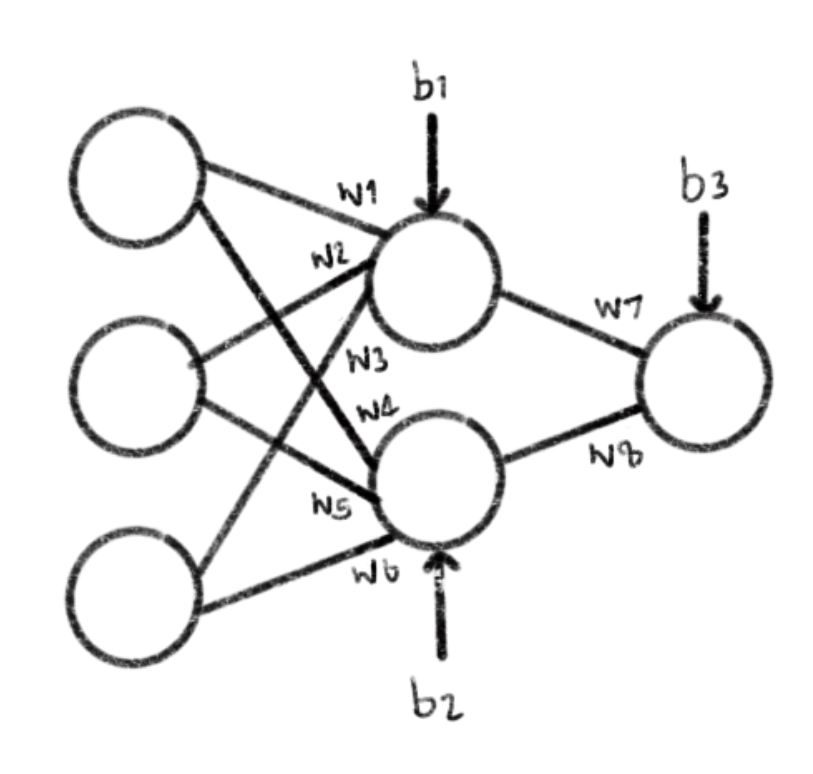
\includegraphics[scale = 0.25]{nn_example.jpg}
    \caption{The 3-2-1 network.}
    \label{fig:1}
\end{figure}
\subsection*{Fitness Function}\label{fitness}
We use both accuracy and mean squared error as the fitness value following the equation \cref*{eq:1} where $i$ is the individual
and $\text{accuracy}_i$, $\text{MSE}_i$ are that individual accuracy and MSE from running through the full training set. 
\begin{equation}\label{eq:1}
f(i) = \text{accuracy}_i + \frac{0.001}{\text{MSE}}_i
\end{equation}
\subsection*{Selection}\label{select}
We use the binary deterministic tournament with reinsertion (implementation on \ref{src:select}) 
as the selection method to select and clone 25 individual to mating pool. 

\subsection*{Crossover}\label{mating}
We random 2 parent from mating pool to be dad and mom, them perforrm a crossover by doing a modified 
uniform crossover with $p_{at\_i} = 0.5$ (\cite{sansanee} page 113) that only produce 1 child with each position on chrosome 
has an equal chance to be from dad or mom (implementation on \ref{src:ga}). We will perform crossover untill we have 25 children for
$P^2$.

\subsection*{Mutation}\label{mutate}
We use strong mutation (\cite{sansanee} page 114) with $p_m = 0.02$ on randomly selected 20 individuals from $P^2$ 
(implementation on \ref{src:ga}).

\subsection*{Full Process}\
Using 10\% cross-validation, and only preprocess each iteration training and validation set with min-max normalization 
to avoid data leakage as state on \cite{dataleak}. The min-max normalization process is done by for each feature $F$ on training set
we find $max(F)$ and $min(F)$ then for each datapoint $F_x$ we compute new datapoint on both training set and 
validation set $F_x' = \frac{F_x - min(F)}{max(F) - min(F)}$, this will guarantee that we applied the min-max normalization using $min$
and $max$ from training set on both training set and validation set. Next, for each cross-validation iteration we follow these steps
(implementation on \ref{src:wdbc}):
\begin{enumerate}
    \item Initialize the population as state on \nameref{init}
    \item For each individual on population we evaluate its fitness as state on \nameref{fitness} and mark the individual that 
    has the largest fitness.
    \item We then process through \nameref{select}, \nameref{mating}, and \nameref{mutate} to get 20 individuals.
    \item For the remaining 5 individual needed, we use clones of the individual that has largest fitness from step 2 to add to the
    population (elitism \cite{sansanee} on page 107).
    \item Repeat step 2-4 untill we fully run through 200 generations and store the individual that has the largest fitness over all 
    generations.
    \item Use that individual from step 5 to test on training and validation set.
\end{enumerate}

\section*{Training Result}\label{trainres}
We will experiment with 3 models which are wdbc-30-15-1, wdbc-30-7-1, and wdbc-30-15-7-1 to see if their training result will have 
any significant differences in training time and accuracy (implementation on \ref{src:wdbc} 
and we use rust compiler with release profile to build and run all trainings). 

\begin{itemize}
    \item {\textbf{wdbc-30-15-1} : The base model that contains 30 input nodes, 1 hidden layer with 15 nodes, 
        and 1 output node with all nodes using sigmoid as an activation function. 
        We assume that this model will have accuracy $ > 95\%$ with reasonable training time used.
        The result is shown on \cref{fig:2}.
    }
    \item{\textbf{wdbc-30-7-1} : A smaller model with 30 input nodes, 1 hidden layer with 7 nodes, and 1 output node. 
        We assume that this model will have faster training time but with less accuracy than the wdbc-30-15-1. The result is shown on \cref{fig:3}
    }
    \item{\textbf{wdbc-30-15-7-1} : A larger model with 30 input nodes, 2 hidden layers with 15 and 7 nodes, and 1 output node.
        We assume that this model will have accuracy $ > 98\%$ with longer training used than the wdbc-30-15-1. The result is shown on \cref{fig:4}
    }
\end{itemize}

\begin{figure}[ht]
    \begin{subfigure}{\textwidth}  
        \centering
        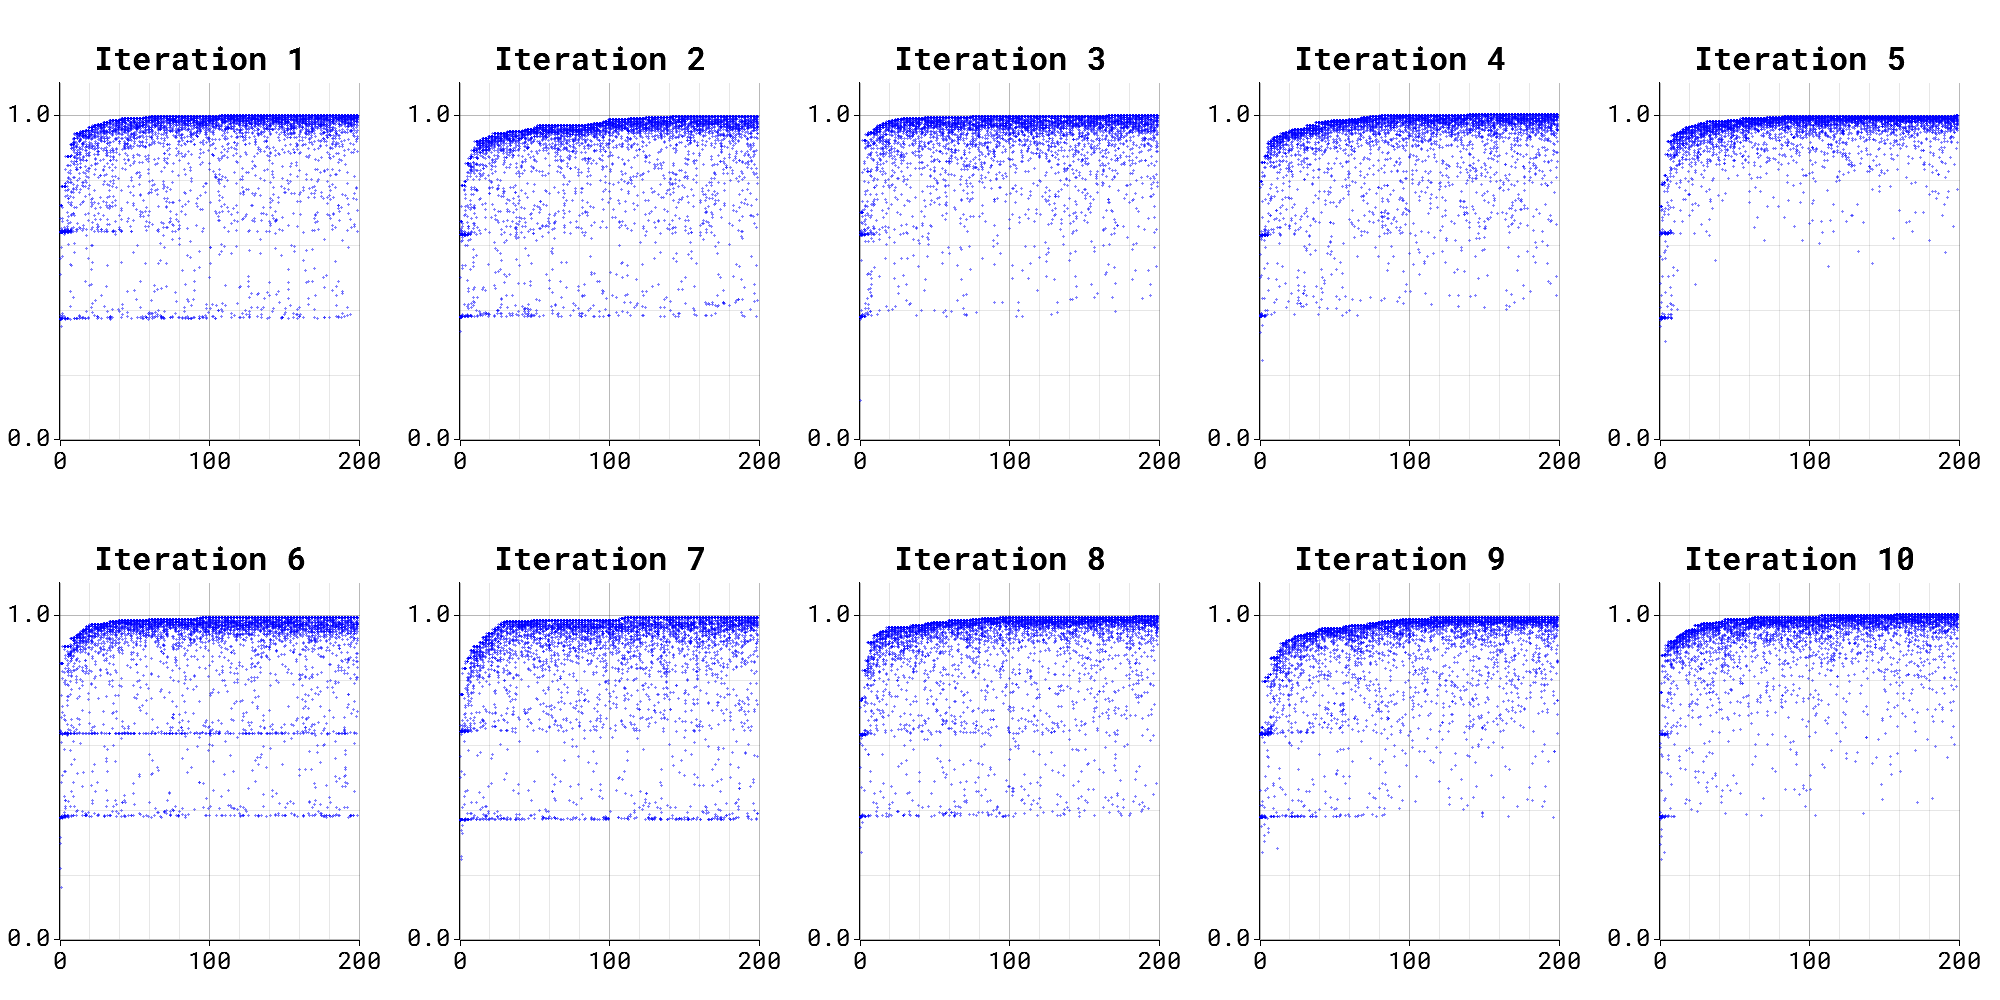
\includegraphics[width=0.89\textwidth]{wdbc-30-15-1/train_proc}
        \caption{The training process of each cross-valiation iteration: x-axis is the generation, y-axis is the fitness value, and each blue dot is an individual in x generation with y fitness.}
        \label{fig:2a}
    \end{subfigure}
    \begin{subfigure}{\textwidth}  
        \centering
        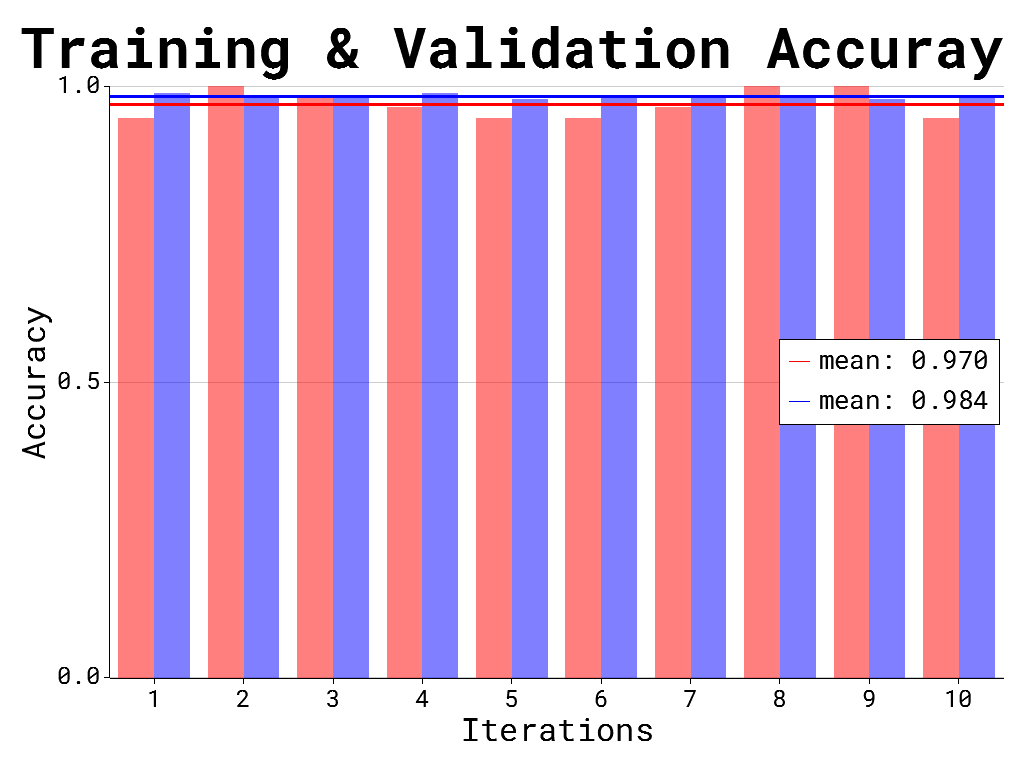
\includegraphics[scale=0.25]{wdbc-30-15-1/accuracy}
        \caption{The best individual from each cross-validation iteration accuracy on training set (blue) and validation set (red).}
        \label{fig:2b}
    \end{subfigure}
    \begin{subfigure}{\textwidth}   
        \centering
        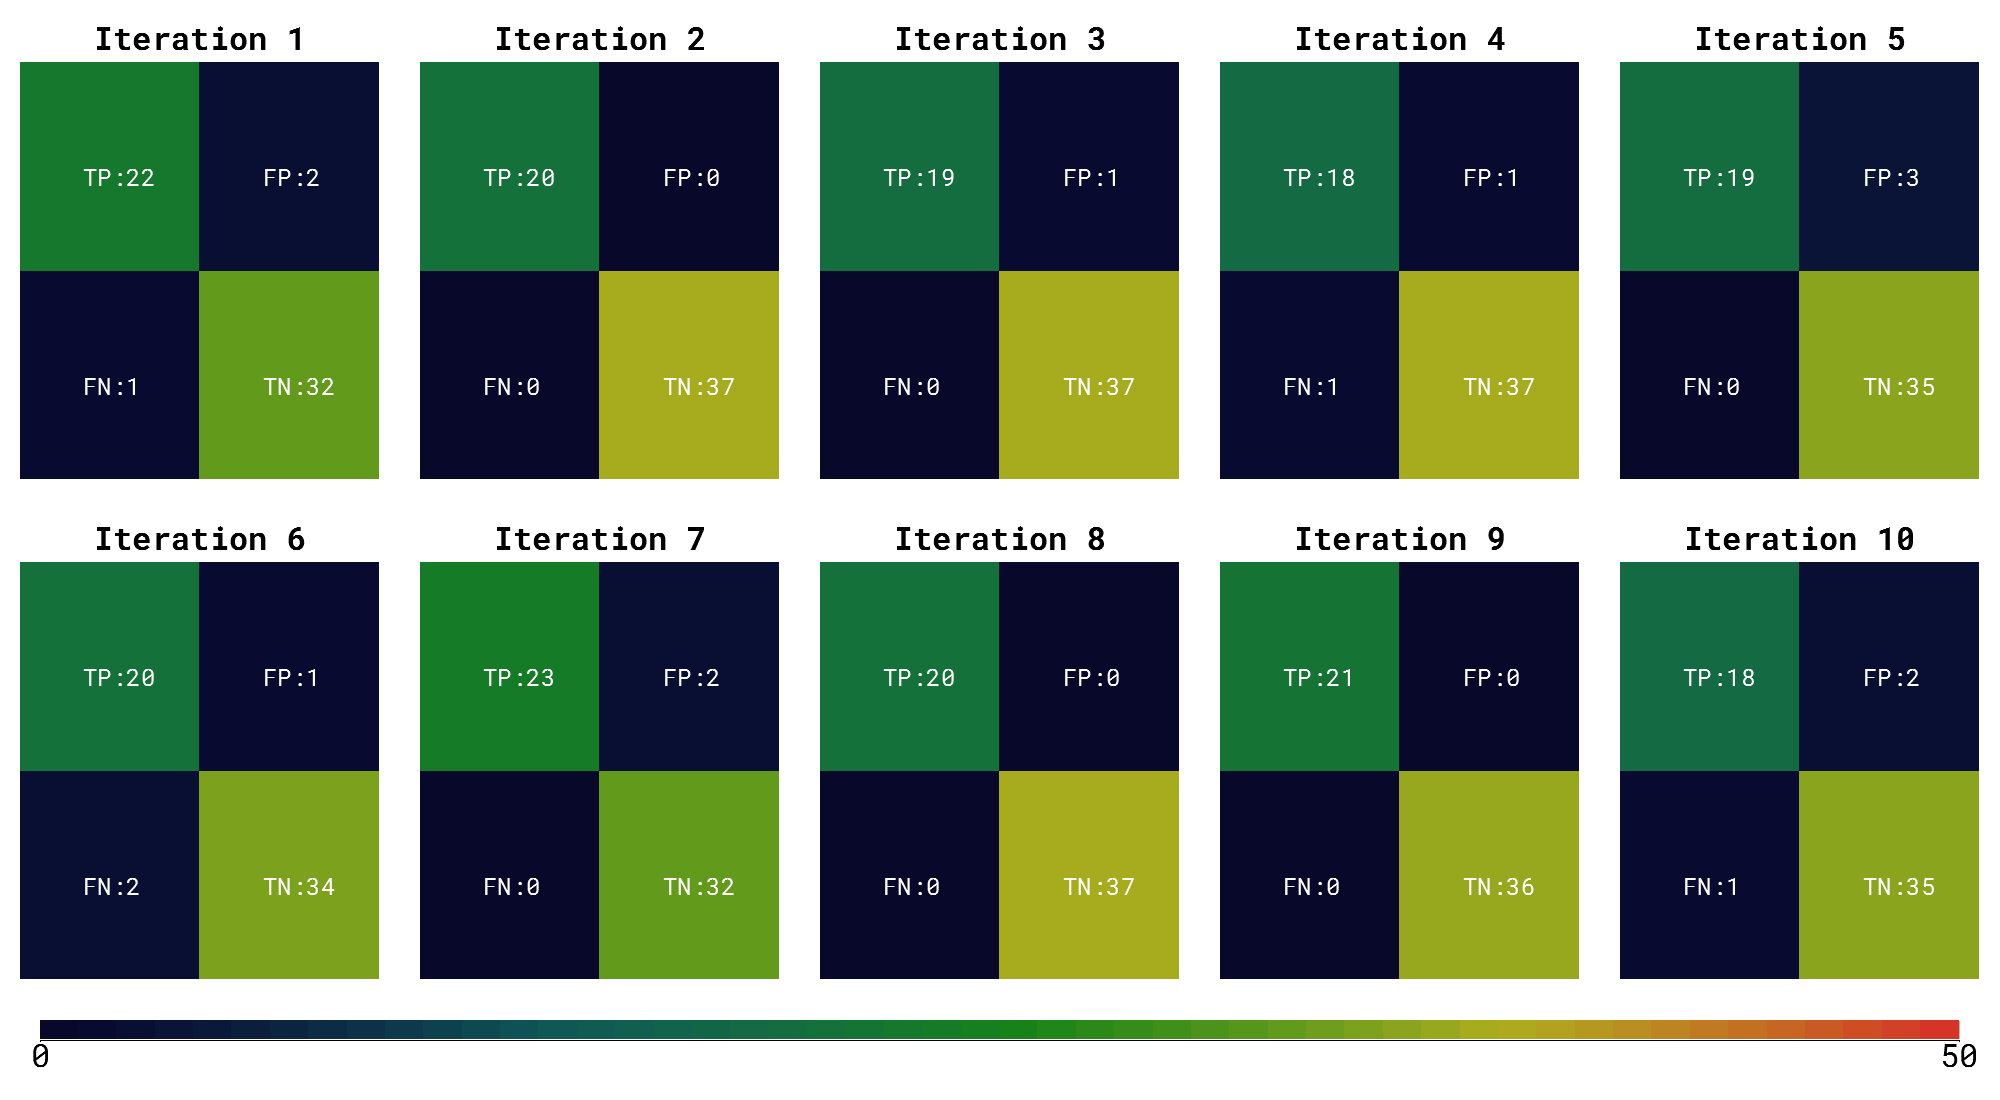
\includegraphics[width=0.89\textwidth]{wdbc-30-15-1/conf_mat}
        \caption{The best individual from each cross-valiation iteration confusion matrix on validation set.}
        \label{fig:2c}
    \end{subfigure}
    \caption{Training result of wdbc-30-15-1 with 20.609 seconds used for training.}
    \label{fig:2}
\end{figure}
\FloatBarrier

\begin{figure}[ht]
    \begin{subfigure}{\textwidth}  
        \centering
        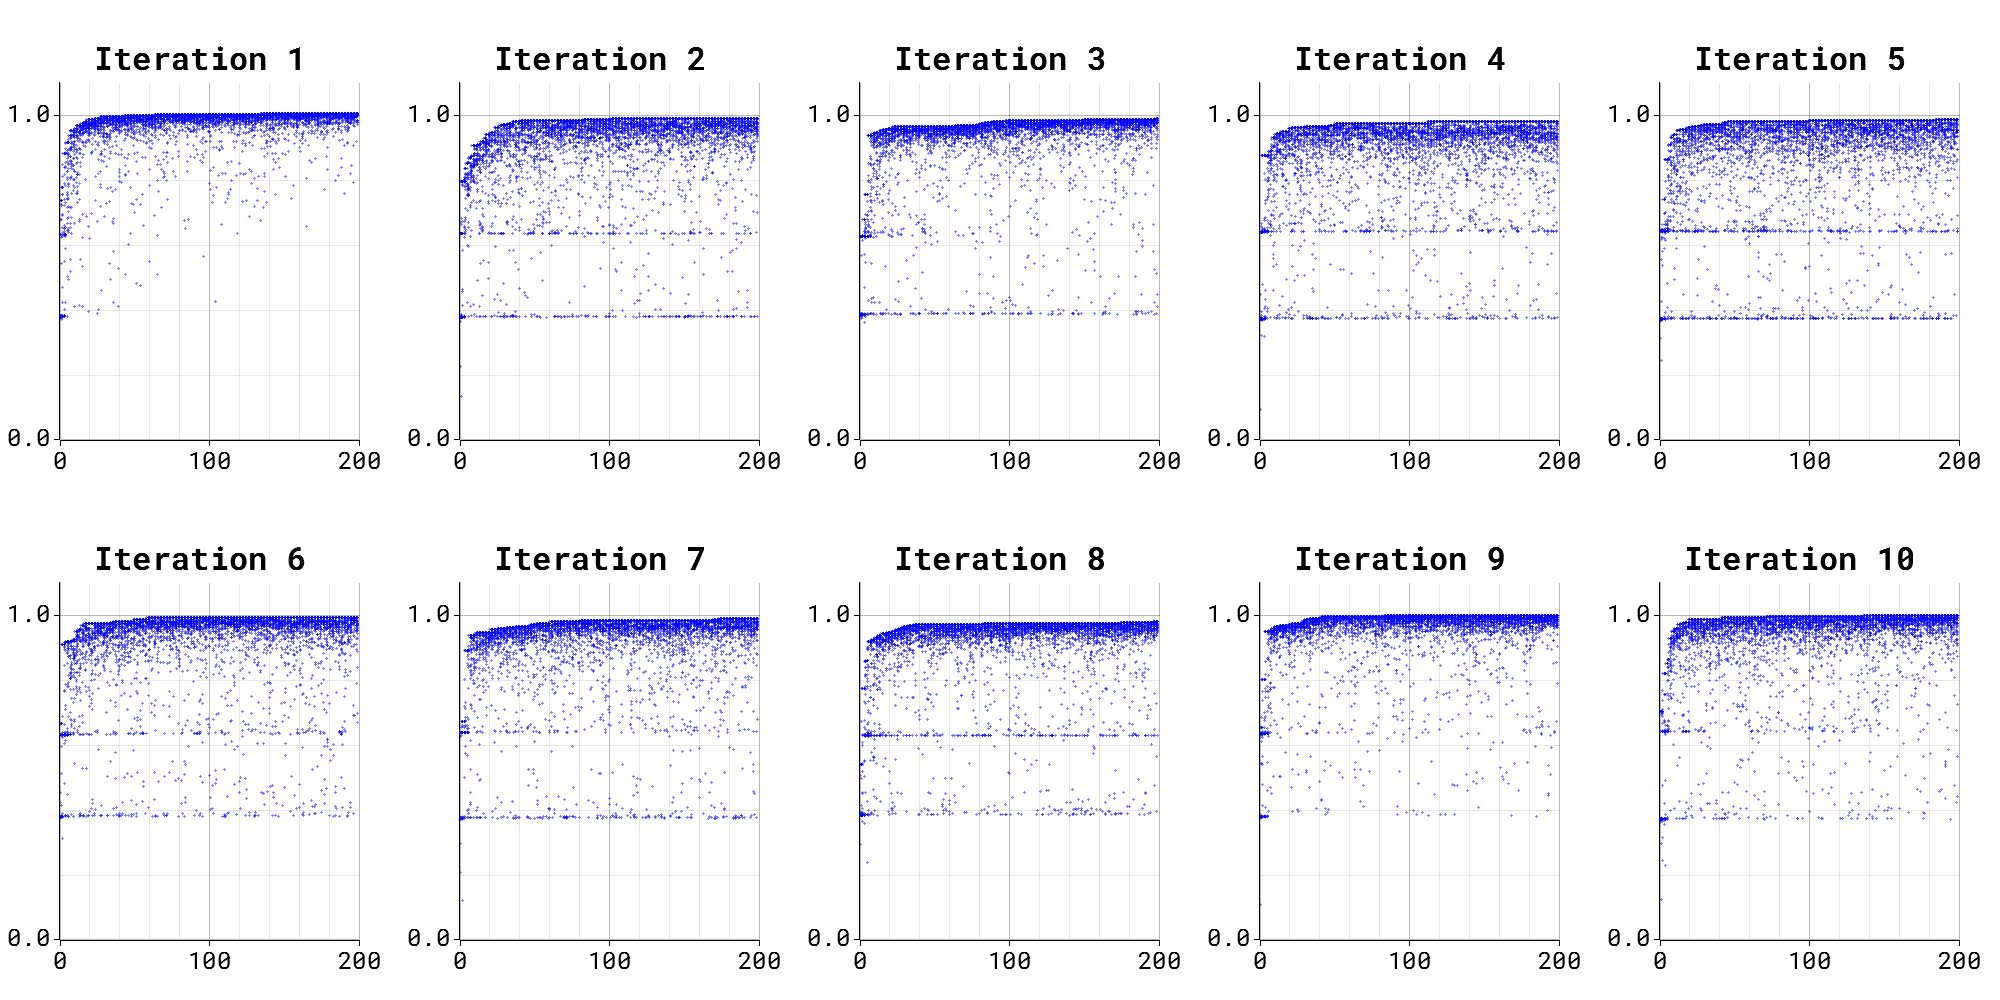
\includegraphics[width=0.89\textwidth]{wdbc-30-7-1/train_proc}
        \caption{The training process of each cross-valiation iteration: x-axis is the generation, y-axis is the fitness value, and each blue dot is an individual in x generation with y fitness.}
        \label{fig:3a}
    \end{subfigure}
    \begin{subfigure}{\textwidth}  
        \centering
        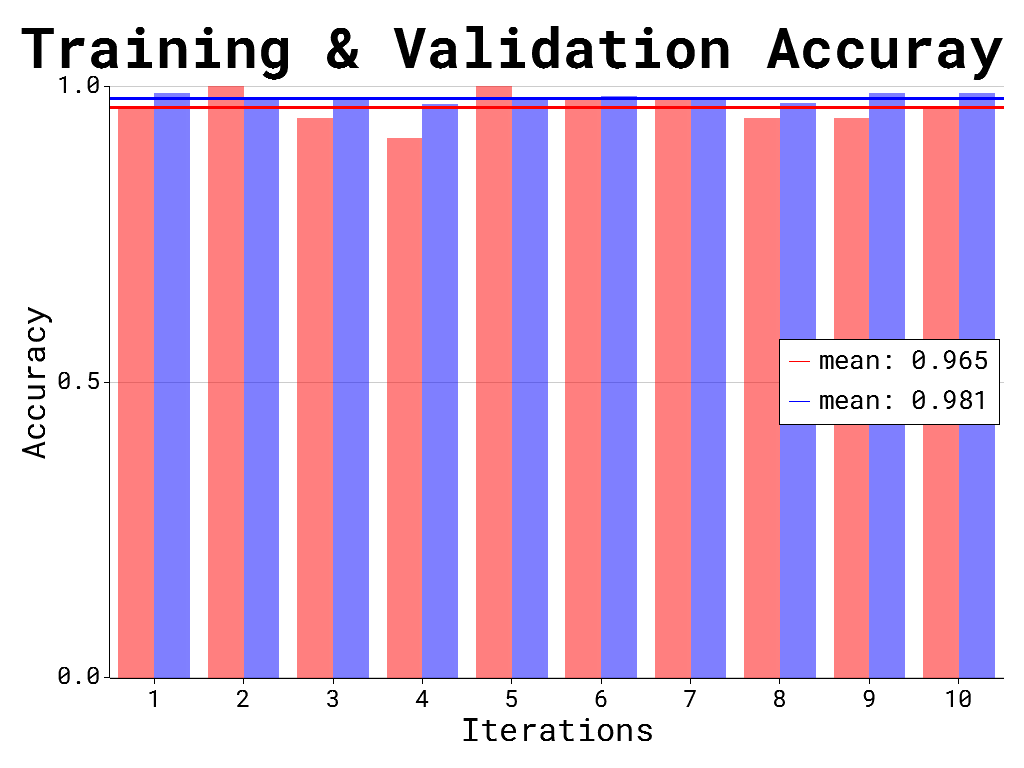
\includegraphics[scale=0.25]{wdbc-30-7-1/accuracy}
        \caption{The best individual from each cross-validation iteration accuracy on training set (blue) and validation set (red).}
        \label{fig:3b}
    \end{subfigure}
    \begin{subfigure}{\textwidth}   
        \centering
        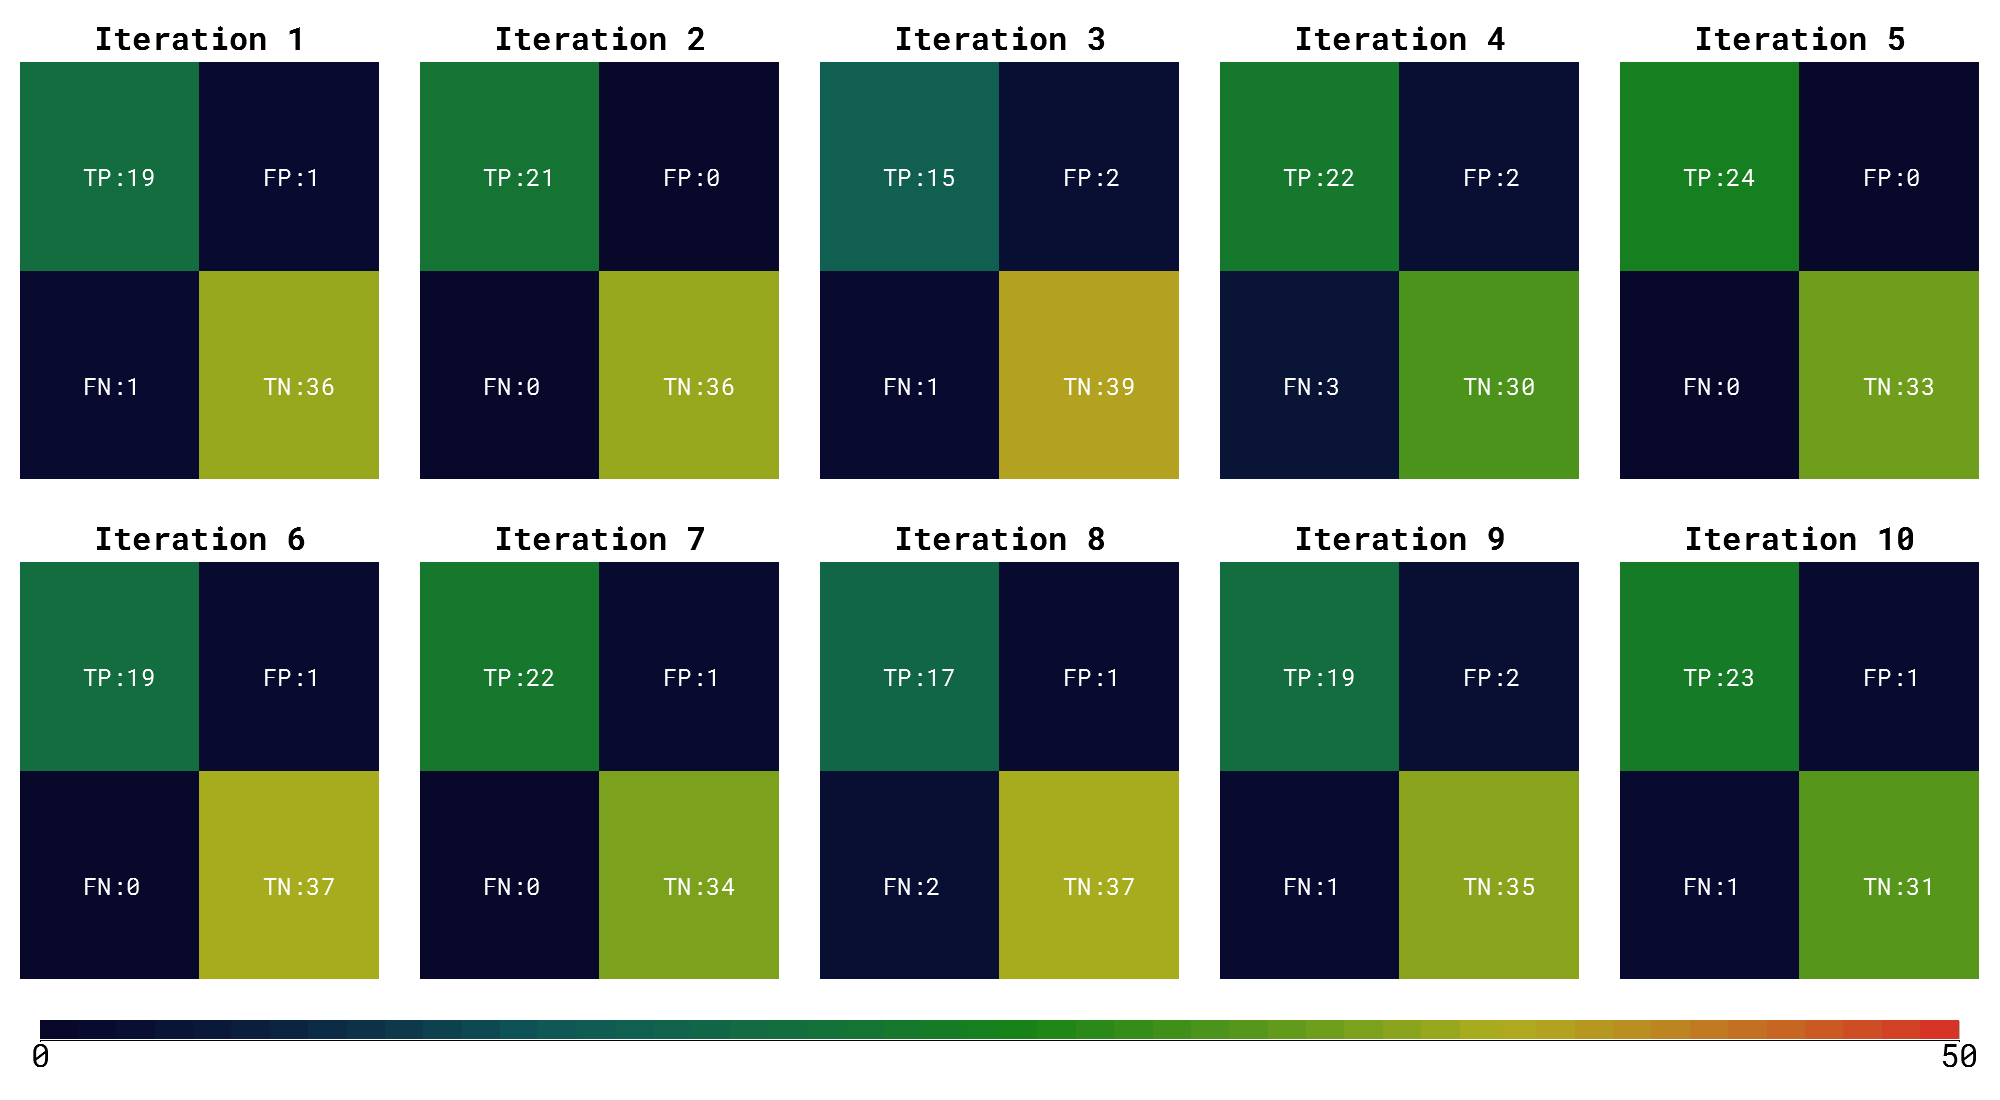
\includegraphics[width=0.89\textwidth]{wdbc-30-7-1/conf_mat}
        \caption{The best individual from each cross-valiation iteration confusion matrix on validation set.}
        \label{fig:3c}
    \end{subfigure}
    \caption{Training result of wdbc-30-7-1 with 14.163 seconds used for training.}
    \label{fig:3}
\end{figure}
\FloatBarrier

\begin{figure}[ht]
    \begin{subfigure}{\textwidth}  
        \centering
        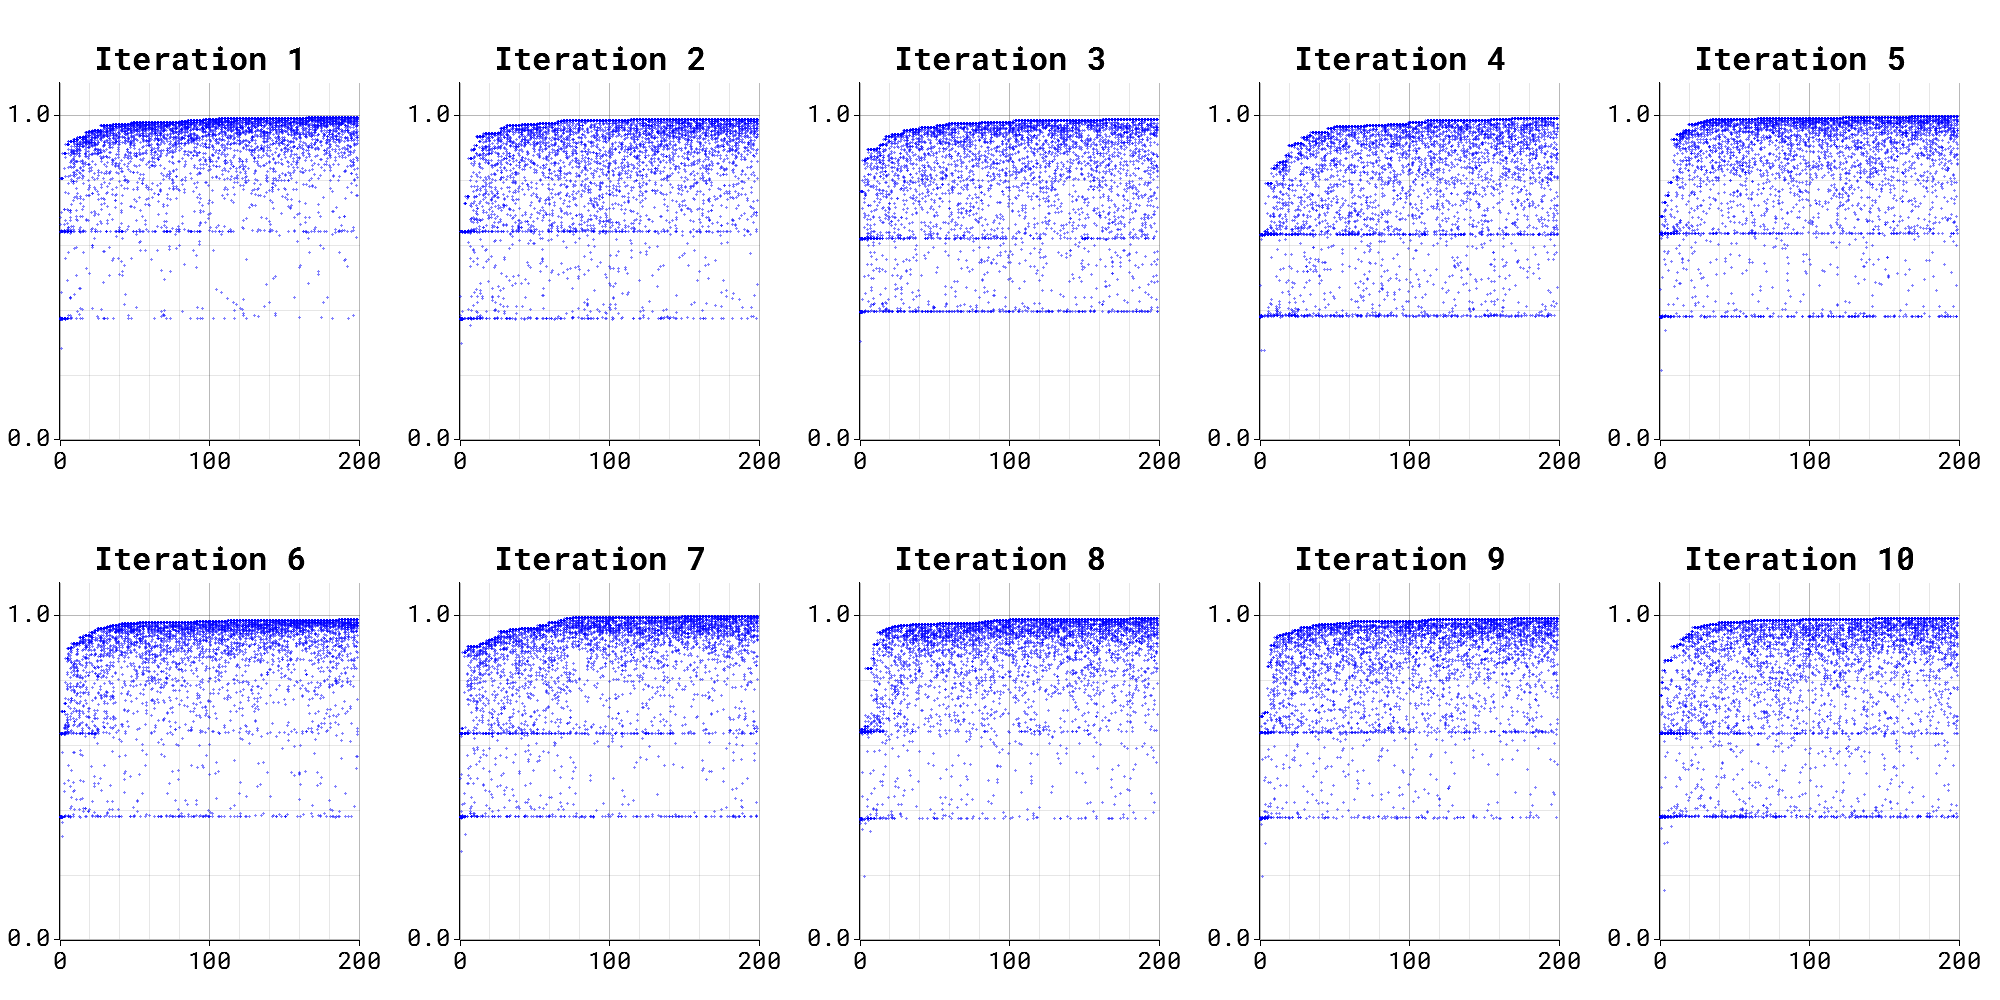
\includegraphics[width=0.89\textwidth]{wdbc-30-15-7-1/train_proc}
        \caption{The training process of each cross-valiation iteration: x-axis is the generation, y-axis is the fitness value, and each blue dot is an individual in x generation with y fitness.}
        \label{fig:4a}
    \end{subfigure}
    \begin{subfigure}{\textwidth}  
        \centering
        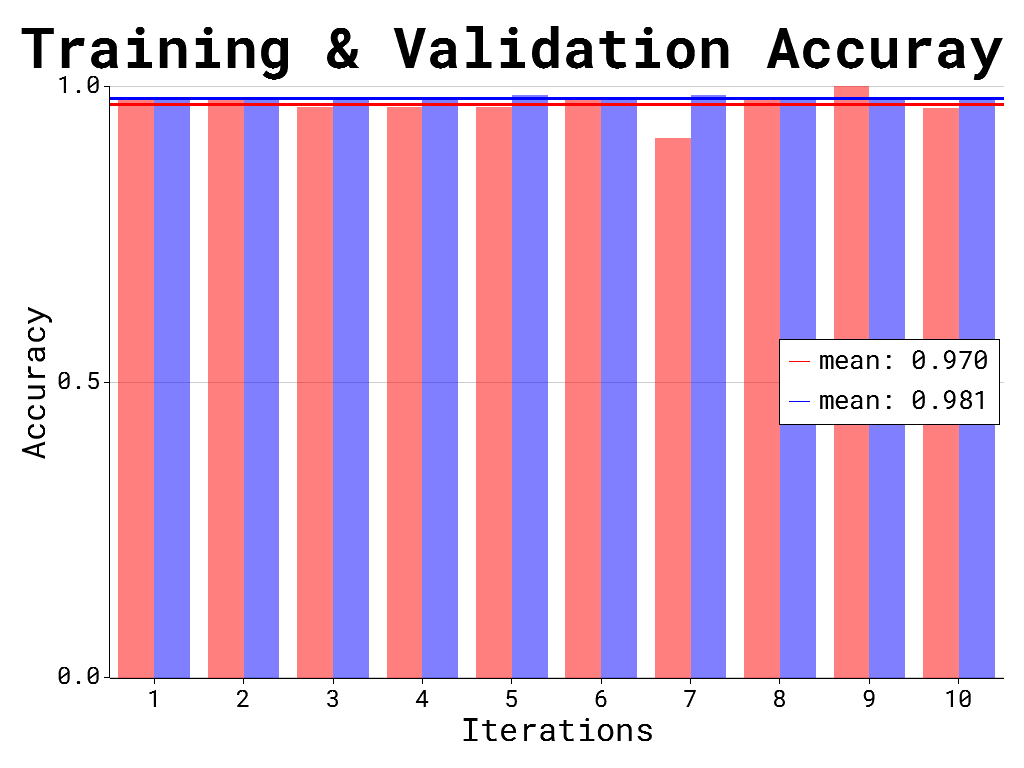
\includegraphics[scale=0.25]{wdbc-30-15-7-1/accuracy}
        \caption{The best individual from each cross-validation iteration accuracy on training set (blue) and validation set (red).}
        \label{fig:4b}
    \end{subfigure}
    \begin{subfigure}{\textwidth}   
        \centering
        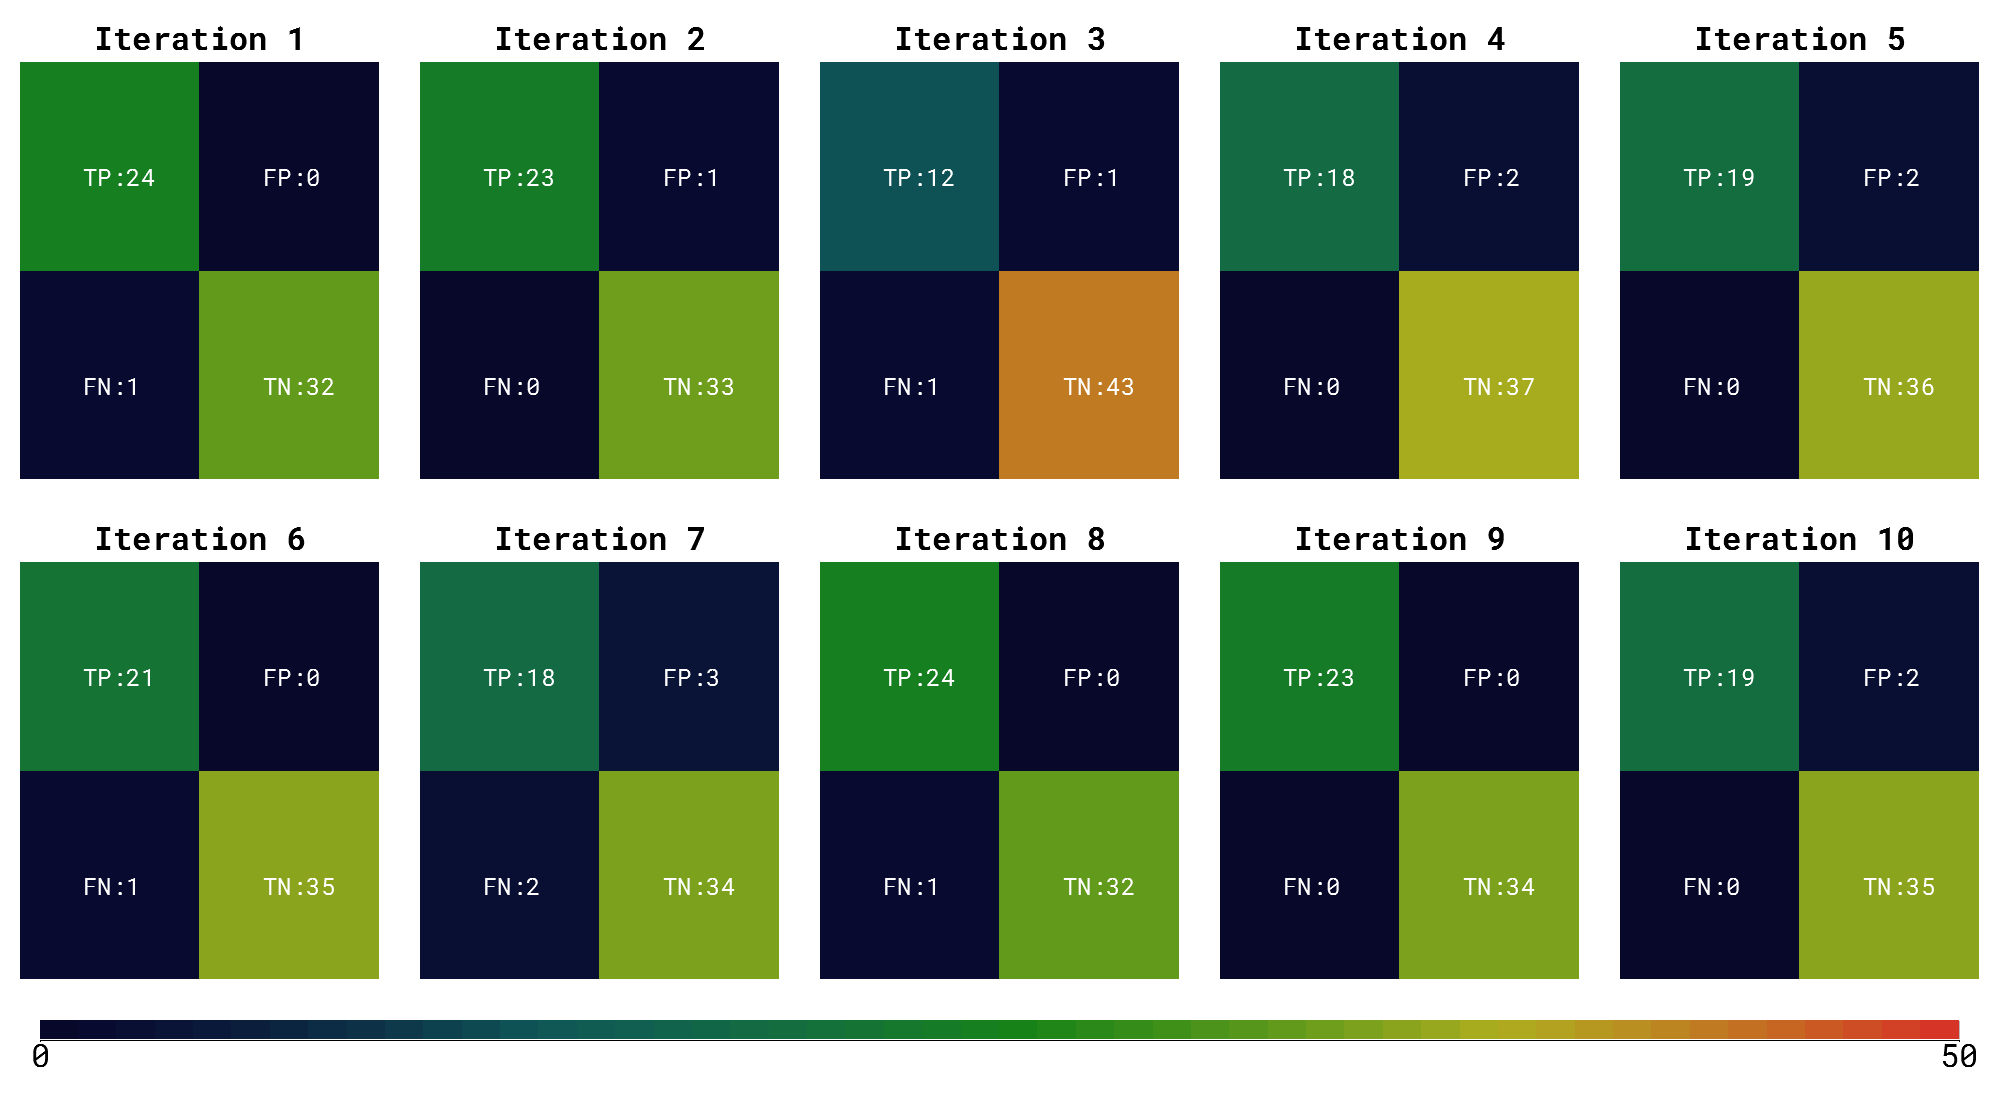
\includegraphics[width=0.89\textwidth]{wdbc-30-15-7-1/conf_mat}
        \caption{The best individual from each cross-valiation iteration confusion matrix on validation set.}
        \label{fig:4c}
    \end{subfigure}
    \caption{Training result of wdbc-30-15-7-1 with 24.244 seconds used for training.}
    \label{fig:4}
\end{figure}
\FloatBarrier

\section*{Analysis}
From \cref{table:1}, we can we that there are no significant accuracy differences in every model which is not matching with our assumption. 
The reason may be that the wdbc dataset is not complex enough for the model that is larger than wdbc-30-7-1. However, the training
time used for every model matches our assumption that wdbc-30-7-1 use the least time and wdbc-30-15-7-1 uses the most time. 
Next, we can see the convergence speed of each model on \cref{fig:2a}, \cref{fig:3a}, and \cref{fig:4a} which for all model the 
best individual seems to reach fitness value near 1.0 in less than 100 generations. Also, the fitness value around 1.0 seems to be 
the barrier for every model which the reason should be because of our fitness function that uses both accuracy and MSE to help with 
the overfitting problem when looking only at MSE (backpropagation method).

\begin{table}[htp]
	\centering
	\begin{tabular}{l S[table-format=2.3] S[table-format=2.1]}
		\toprule
        \multicolumn{1}{c}{Model} & {Training Time (seconds)} & {Validation Set Mean Accuracy (\%)} \\
        \midrule
        wdbc-30-15-1 & 20.609 & 97.0 \\
        wdbc-30-7-1 & 14.163 & 96.5 \\
        wdbc-30-15-7-1 & 24.244 & 97.0 \\
        \bottomrule
    \end{tabular} 
	\caption{Training time and validation set mean accuracy (red line on 
		\cref{fig:2b}, \cref{fig:3b}, and \cref{fig:4b}) of each model.}
	\label{table:1}
\end{table}

\section*{Summary}
Genetic Algorithm (GA) is an okay algorithm to use for training MLP if we know how we should design a fitness function and how to 
implement GA with efficiency. GA can train MLP to create a model that is usable as we demonstrated on \nameref{trainres}. 
Rust language is also a great tool for implementing GA because of how fast it is and how easy it is to write a memory-safe program.

\printbibliography

\definecolor{bg}{rgb}{0.97,0.97,0.98}

\section*{Appendix}
main.rs
\begin{minted}[fontsize=\footnotesize, bgcolor=bg]{rust}
pub mod activator;
pub mod cross;
pub mod flood;
pub mod loss;
pub mod model;
pub mod utills;

use std::error::Error;

fn main() -> Result<(), Box<dyn Error>> {
    // training code
    flood::flood_8_4_1(0.01, 0.01, "flood-8-4-1", true)?; // base
    flood::flood_8_4_1(0.01, 0.0, "flood-8-4-1_2", true)?; // no momentum
    flood::flood_8_4_1(0.0001, 0.01, "flood-8-4-1_3", true)?; // small learning rate
    flood::flood_8_4_1(0.01, 0.01, "flood-8-4-1_4", false)?; // no data preprocessing
    flood::flood_8_8_1(0.01, 0.01, "flood-8-8-1")?; 

    cross::cross_2_4_1(0.01, 0.01, "cross-2-4-1")?; // base
    cross::cross_2_4_1(0.01, 0.0, "cross-2-4-1_2")?; // no momentum
    cross::cross_2_4_1(0.0001, 0.01, "cross-2-4-1_3")?; // small learning rate
    cross::cross_2_8_1(0.01, 0.01, "cross-2-8-1")?;

    Ok(())
}
\end{minted}
\noindent flood/mod.rs
\begin{minted}[fontsize=\footnotesize, bgcolor=bg]{rust}
    //! Contains training code for variations of flood dataset models.
    use super::activator;
    use super::loss;
    use super::model;
    use super::utills;
    
    use model::{Layer, Net};
    use std::error::Error;
    use std::fs;
    use std::io::Write;
    use std::time::{Duration, Instant};
    use utills::data;
    use utills::graph;
    use utills::io;
    
    pub fn flood_8_4_1(
        lr: f64,
        momentum: f64,
        folder: &str,
        standardize: bool,
    ) -> Result<(), Box<dyn Error>> {
        fn model() -> Net {
            let mut layers: Vec<model::Layer> = vec![];
            layers.push(Layer::new(8, 4, 1.0, activator::sigmoid()));
            layers.push(Layer::new(4, 1, 1.0, activator::linear()));
            Net::from_layers(layers)
        }
    
        flood_fit(&model, lr, momentum, folder, standardize)?;
        Ok(())
    }
    
    pub fn flood_8_8_1(lr: f64, momentum: f64, folder: &str) -> Result<(), Box<dyn Error>> {
        fn model() -> Net {
            let mut layers: Vec<model::Layer> = vec![];
            layers.push(Layer::new(8, 8, 1.0, activator::sigmoid()));
            layers.push(Layer::new(8, 1, 1.0, activator::linear()));
            Net::from_layers(layers)
        }
    
        flood_fit(&model, lr, momentum, folder, true)?;
        Ok(())
    }
    
    fn mse_to_rmse(mse: &Vec<f64>) -> Vec<f64> {
        mse.iter().map(|v| v.sqrt()).collect()
    }
    
    pub fn flood_fit(
        model: &dyn Fn() -> Net,
        lr: f64,
        momentum: f64,
        folder: &str,
        standardize: bool,
    ) -> Result<(), Box<dyn Error>> {
        let (models, img) = utills::io::check_dir(folder)?;
    
        let dataset = data::flood_dataset()?;
        let mut loss = loss::Loss::mse();
        let epochs = 1000;
    
        let mut cv_valid_loss: Vec<f64> = vec![];
        let mut cv_train_loss: Vec<f64> = vec![];
    
        let mut r2_score: Vec<f64> = vec![];
        let mut loss_g = graph::LossGraph::new();
        let start = Instant::now();
        for (j, dt) in dataset.cross_valid_set(0.1).iter().enumerate() {
            // creating a model
            let mut net = model();
    
            // get training set and validation set
            let training_set = if standardize {
                data::standardization(&dt.0, dt.0.mean(), dt.0.std())
            } else {
                dt.0.clone()
            };
    
            let validation_set = if standardize {
                data::standardization(&dt.1, dt.0.mean(), dt.0.std())
            } else {
                dt.1.clone()
            };
            //let training_set = data::minmax_norm(&dt.0, dt.0.min(), dt.0.max());
            //let validation_set = data::minmax_norm(&dt.1, dt.1.min(), dt.1.max());
    
            // training
            let mut loss_vec: Vec<f64> = vec![];
            let mut valid_loss_vec: Vec<f64> = vec![];
            for i in 0..epochs {
                let mut running_loss: f64 = 0.0;
    
                for data in training_set.get_shuffled() {
                    let result = net.forward(&data.inputs);
    
                    running_loss += loss.criterion(&result, &data.labels);
                    loss.backward(&mut net.layers);
    
                    net.update(lr, momentum);
                }
                running_loss /= training_set.len() as f64;
                loss_vec.push(running_loss);
    
                let mut valid_loss: f64 = 0.0;
                for data in validation_set.get_datas() {
                    let result = net.forward(&data.inputs);
                    valid_loss += loss.criterion(&result, &data.labels);
                }
                valid_loss /= validation_set.get_datas().len() as f64;
                valid_loss_vec.push(valid_loss);
    
                if i == epochs - 1 {
                    // log score
                    let label_mean = validation_set.get_datas().iter().fold(0f64, |mean, val| {
                        mean + val.labels[0] / validation_set.len() as f64
                    });
    
                    let mut total_sum_sqr = 0f64;
                    let mut sum_sqr = 0f64;
    
                    for data in validation_set.get_datas() {
                        let result = net.forward(&data.inputs);
                        sum_sqr += (data.labels[0] - result[0]).powi(2);
                        total_sum_sqr += (data.labels[0] - label_mean).powi(2);
                    }
    
                    r2_score.push(1.0 - (sum_sqr / total_sum_sqr));
                    cv_valid_loss.push(valid_loss);
                    cv_train_loss.push(running_loss);
                }
    
                println!(
                    "iteration: {}, epoch: {}, loss: {:.6}, valid_loss: {:.6}",
                    j, i, running_loss, valid_loss
                );
            }
    
            loss_g.add_loss(loss_vec, valid_loss_vec);
            io::save(&net.layers, format!("{}/{}.json", models, j))?;
        }
        let duration: Duration = start.elapsed();
    
        let mut file = fs::File::create(format!("{}/result.txt", models))?;
        file.write_all(
            format!(
                "cv_score: {:?}\n\nr2_score: {:?}\n\ntime used: {:?}",
                cv_valid_loss, r2_score, duration
            )
            .as_bytes(),
        )?;
    
        loss_g.draw(format!("{}/loss.png", img))?;
    
        graph::draw_2hist(
            [mse_to_rmse(&cv_valid_loss), mse_to_rmse(&cv_train_loss)],
            "Validation/Training RMSE",
            ("Iterations", "Validataion/Training RMSE"),
            format!("{}/cv_l.png", img),
        )?;
    
        graph::draw_histogram(
            r2_score,
            "Cross Validation R2 Scores",
            ("Iterations", "R2 Scores"),
            format!("{}/r2_score.png", img),
        )?;
        Ok(())
    }
\end{minted}
\noindent cross/mod.rs
\begin{minted}[fontsize=\footnotesize, bgcolor=bg]{rust}
//! Contains training code for variations of cross.pat dataset models.
use super::activator;
use super::loss;
use super::model;
use super::utills;

use model::{Layer, Net};
use std::error::Error;
use std::fs;
use std::io::Write;
use std::time::{Duration, Instant};
use utills::data;
use utills::graph;
use utills::io;

fn confusion_count(matrix: &mut [[i32; 2]; 2], result: &Vec<f64>, label: &Vec<f64>) {
    let threshold = 0.5;
    if result[0] > threshold {
        // true positive
        if label[0] == 1.0 {
            matrix[0][0] += 1
        } else {
            // false negative
            matrix[1][0] += 1
        }
    } else if result[0] <= threshold {
        // true negative
        if label[0] == 0.0 {
            matrix[1][1] += 1
        }
        // false positive
        else {
            matrix[0][1] += 1
        }
    }
}

pub fn cross_2_4_1(lr: f64, momentum: f64, folder: &str) -> Result<(), Box<dyn Error>> {
    fn model() -> Net {
        let mut layers: Vec<model::Layer> = vec![];
        layers.push(Layer::new(2, 4, 1.0, activator::sigmoid()));
        layers.push(Layer::new(4, 1, 1.0, activator::sigmoid()));
        Net::from_layers(layers)
    }

    cross_fit(&model, lr, momentum, folder)?;
    Ok(())
}

pub fn cross_2_8_1(lr: f64, momentum: f64, folder: &str) -> Result<(), Box<dyn Error>> {
    fn model() -> Net {
        let mut layers: Vec<model::Layer> = vec![];
        layers.push(Layer::new(2, 8, 1.0, activator::sigmoid()));
        layers.push(Layer::new(8, 1, 1.0, activator::sigmoid()));
        Net::from_layers(layers)
    }

    cross_fit(&model, lr, momentum, folder)?;
    Ok(())
}

pub fn cross_fit(
    model: &dyn Fn() -> Net,
    lr: f64,
    momentum: f64,
    folder: &str,
) -> Result<(), Box<dyn Error>> {
    let (models, img) = utills::io::check_dir(folder)?;

    let dataset = data::cross_dataset()?;
    let mut loss = loss::Loss::mse();
    let epochs = 7500;

    let mut valid_acc: Vec<f64> = vec![];
    let mut train_acc: Vec<f64> = vec![];
    let mut loss_g = graph::LossGraph::new();
    let mut matrix_vec: Vec<[[i32; 2]; 2]> = vec![];

    let start = Instant::now();
    for (j, dt) in dataset.cross_valid_set(0.1).iter().enumerate() {
        // creating a model
        let mut net = model();

        // get training set and validation set
        let training_set = &dt.0;
        let validation_set = &dt.1;

        // training
        let mut loss_vec: Vec<f64> = vec![];
        let mut valid_loss_vec: Vec<f64> = vec![];
        for i in 0..epochs {
            let mut running_loss: f64 = 0.0;

            for data in training_set.get_shuffled() {
                let result = net.forward(&data.inputs);

                running_loss += loss.criterion(&result, &data.labels);
                loss.backward(&mut net.layers);

                net.update(lr, momentum);
            }
            running_loss /= training_set.len() as f64;
            loss_vec.push(running_loss);

            let mut valid_loss: f64 = 0.0;
            for data in validation_set.get_datas() {
                let result = net.forward(&data.inputs);
                valid_loss += loss.criterion(&result, &data.labels);
            }
            valid_loss /= validation_set.get_datas().len() as f64;
            valid_loss_vec.push(valid_loss);

            if i == epochs - 1 {
                let mut matrix = [[0, 0], [0, 0]];
                for data in validation_set.get_datas() {
                    let result = net.forward(&data.inputs);
                    confusion_count(&mut matrix, &result, &data.labels);
                }

                let mut matrix2 = [[0, 0], [0, 0]];
                for data in training_set.get_datas() {
                    let result = net.forward(&data.inputs);
                    confusion_count(&mut matrix2, &result, &data.labels);
                }
                valid_acc.push((matrix[0][0] + matrix[1][1]) as f64 / validation_set.len() as f64);
                train_acc.push((matrix2[0][0] + matrix2[1][1]) as f64 / training_set.len() as f64);
                matrix_vec.push(matrix);
            }

            println!(
                "iteration: {}, epoch: {}, loss: {:.6}, valid_loss: {:.6}",
                j, i, running_loss, valid_loss
            );
        }

        loss_g.add_loss(loss_vec, valid_loss_vec);
        io::save(&net.layers, format!("{}/{}.json", models, j))?;
    }
    let duration: Duration = start.elapsed();

    let mut file = fs::File::create(format!("{}/result.txt", models))?;
    file.write_all(format!("cv_score: {:?}\n\ntime used: {:?}", valid_acc, duration).as_bytes())?;

    loss_g.draw(format!("{}/loss.png", img))?;

    graph::draw_2hist(
        [valid_acc, train_acc],
        "Validation/Training Accuracy",
        ("Iterations", "Validataion/Training Accuracy"),
        format!("{}/acc.png", img),
    )?;

    graph::draw_confustion(matrix_vec, format!("{}/confusion_matrix.png", img))?;

    Ok(())
}
\end{minted}
\noindent model.rs
\begin{minted}[fontsize=\footnotesize, bgcolor=bg]{rust}
    use crate::activator;

    #[derive(Debug)]
    pub struct Layer {
        pub inputs: Vec<f64>,
        pub outputs: Vec<f64>, // need to save this for backward pass
        pub w: Vec<Vec<f64>>,
        pub b: Vec<f64>,
        pub grads: Vec<Vec<f64>>,
        pub w_prev_changes: Vec<Vec<f64>>,
        pub local_grads: Vec<f64>,
        pub b_prev_changes: Vec<f64>,
        pub act: activator::ActivationContainer,
    }
    
    impl Layer {
        pub fn new(
            input_features: u64,
            output_features: u64,
            bias: f64,
            act: activator::ActivationContainer,
        ) -> Layer {
            // initialize weights matrix
            let mut weights: Vec<Vec<f64>> = vec![];
            let mut inputs: Vec<f64> = vec![];
            let mut outputs: Vec<f64> = vec![];
            let mut grads: Vec<Vec<f64>> = vec![];
            let mut local_grads: Vec<f64> = vec![];
            let mut w_prev_changes: Vec<Vec<f64>> = vec![];
            let mut b_prev_changes: Vec<f64> = vec![];
            let mut b: Vec<f64> = vec![];
    
            for _ in 0..output_features {
                outputs.push(0.0);
                local_grads.push(0.0);
                b_prev_changes.push(0.0);
                b.push(bias);
    
                let mut w: Vec<f64> = vec![];
                let mut g: Vec<f64> = vec![];
                for _ in 0..input_features {
                    if (inputs.len() as u64) < input_features {
                        inputs.push(0.0);
                    }
                    g.push(0.0);
                    // random both positive and negative weight
                    w.push(2f64 * rand::random::<f64>() - 1f64);
                }
                weights.push(w);
                grads.push(g.clone());
                w_prev_changes.push(g);
            }
            Layer {
                inputs,
                outputs,
                w: weights,
                b,
                grads,
                w_prev_changes,
                local_grads,
                b_prev_changes,
                act,
            }
        }
    
        pub fn forward(&mut self, inputs: &Vec<f64>) -> Vec<f64> {
            if inputs.len() != self.inputs.len() {
                panic!("forward: input size is wrong");
            }
            let mut result: Vec<f64> = vec![];
            for j in 0..self.outputs.len() {
                let mut sum: f64 = 0.0;
                // loop through input and add w*x + b to sum
                for i in 0..inputs.len() {
                    sum += self.w[j][i] * inputs[i];
                }
                sum += self.b[j];
                self.outputs[j] = sum;
                result.push((self.act.func)(sum));
            }
            self.inputs = inputs.clone();
            result
        }
    
        pub fn update(&mut self, lr: f64, momentum: f64) {
            for j in 0..self.w.len() {
                let delta_b = lr * self.local_grads[j] + momentum * self.b_prev_changes[j];
                self.b[j] -= delta_b; // update each neuron bias
                self.b_prev_changes[j] = delta_b;
                for i in 0..self.w[j].len() {
                    // update each weights
                    let delta_w = lr * self.grads[j][i] + momentum * self.w_prev_changes[j][i];
                    self.w[j][i] -= delta_w;
                    self.w_prev_changes[j][i] = delta_w;
                }
            }
        }
    
        pub fn zero_grad(&mut self) {
            for j in 0..self.outputs.len() {
                self.local_grads[j] = 0.0;
                for i in 0..self.grads[j].len() {
                    self.grads[j][i] = 0.0;
                }
            }
        }
    }
    
    #[derive(Debug)]
    pub struct Net {
        pub layers: Vec<Layer>,
    }
    
    impl Net {
        pub fn from_layers(layers: Vec<Layer>) -> Net {
            Net { layers }
        }
    
        pub fn new(architecture: Vec<u64>) -> Net {
            let mut layers: Vec<Layer> = vec![];
            for i in 1..architecture.len() {
                layers.push(Layer::new(
                    architecture[i - 1],
                    architecture[i],
                    1f64,
                    activator::sigmoid(),
                ))
            }
            Net { layers }
        }
    
        pub fn zero_grad(&mut self) {
            for l in 0..self.layers.len() {
                self.layers[l].zero_grad();
            }
        }
    
        pub fn forward(&mut self, input: &Vec<f64>) -> Vec<f64> {
            let mut result = self.layers[0].forward(input);
            for l in 1..self.layers.len() {
                result = self.layers[l].forward(&result);
            }
            result
        }
    
        pub fn update(&mut self, lr: f64, momentum: f64) {
            for l in 0..self.layers.len() {
                self.layers[l].update(lr, momentum);
            }
        }
    }
    
    #[cfg(test)]
    mod tests {
        use super::*;
    
        #[test]
        fn test_linear_new() {
            let linear = Layer::new(2, 3, 1.0, activator::linear());
            assert_eq!(linear.outputs.len(), 3);
            assert_eq!(linear.inputs.len(), 2);
    
            assert_eq!(linear.w.len(), 3);
            assert_eq!(linear.w[0].len(), 2);
            assert_eq!(linear.b.len(), 3);
    
            assert_eq!(linear.grads.len(), 3);
            assert_eq!(linear.w_prev_changes.len(), 3);
            assert_eq!(linear.grads[0].len(), 2);
            assert_eq!(linear.w_prev_changes[0].len(), 2);
            assert_eq!(linear.local_grads.len(), 3);
            assert_eq!(linear.b_prev_changes.len(), 3);
        }
    
        #[test]
        fn test_linear_forward1() {
            let mut linear = Layer::new(2, 1, 1.0, activator::sigmoid());
    
            for j in 0..linear.w.len() {
                for i in 0..linear.w[j].len() {
                    linear.w[j][i] = 1.0;
                }
            }
    
            assert_eq!(linear.forward(&vec![1.0, 1.0])[0], 0.9525741268224334);
            assert_eq!(linear.outputs[0], 3.0);
        }
    
        #[test]
        fn test_linear_forward2() {
            let mut linear = Layer::new(2, 2, 1.0, activator::sigmoid());
    
            for j in 0..linear.w.len() {
                for i in 0..linear.w[j].len() {
                    linear.w[j][i] = (j as f64) + 1.0;
                }
            }
            let result = linear.forward(&vec![0.0, 1.0]);
            assert_eq!(linear.outputs[0], 2.0);
            assert_eq!(linear.outputs[1], 3.0);
            assert_eq!(result[0], 0.8807970779778823);
            assert_eq!(result[1], 0.9525741268224334);
        }
    }   
\end{minted}
\noindent activator.rs
\begin{minted}[fontsize=\footnotesize, bgcolor=bg]{rust}
#[derive(Debug)]
pub struct ActivationContainer {
    pub func: fn(f64) -> f64,
    pub der: fn(f64) -> f64,
    pub name: String,
}

pub fn sigmoid() -> ActivationContainer {
    fn func(input: f64) -> f64 {
        1.0 / (1.0 + (-input).exp())
    }
    fn der(input: f64) -> f64 {
        func(input) * (1.0 - func(input))
    }
    ActivationContainer {
        func,
        der,
        name: "sigmoid".to_string(),
    }
}

pub fn relu() -> ActivationContainer {
    fn func(input: f64) -> f64 {
        return f64::max(0.0, input);
    }
    fn der(input: f64) -> f64 {
        if input > 0.0 {
            return 1.0;
        } else {
            return 0.0;
        }
    }
    ActivationContainer {
        func,
        der,
        name: "relu".to_string(),
    }
}

pub fn linear() -> ActivationContainer {
    fn func(input: f64) -> f64 {
        input
    }
    fn der(_input: f64) -> f64 {
        1.0
    }
    ActivationContainer {
        func,
        der,
        name: "linear".to_string(),
    }
}

#[cfg(test)]
mod tests {
    use super::*;

    #[test]
    fn test_sigmoid() {
        let act = sigmoid();

        assert_eq!((act.func)(1.0), 0.7310585786300048792512);
        assert_eq!((act.func)(-1.0), 0.2689414213699951207488);
        assert_eq!((act.func)(0.0), 0.5);
        assert_eq!((act.der)(1.0), 0.1966119332414818525374);
        assert_eq!((act.der)(-1.0), 0.1966119332414818525374);
        assert_eq!((act.der)(0.0), 0.25);
    }

    #[test]
    fn test_relu() {
        let act = relu();

        assert_eq!((act.func)(-1.0), 0.0);
        assert_eq!((act.func)(20.0), 20.0);
        assert_eq!((act.der)(-1.0), 0.0);
        assert_eq!((act.der)(20.0), 1.0);
    }
}

\end{minted}
\noindent loss.rs
\begin{minted}[fontsize=\footnotesize, bgcolor=bg]{rust}    
use crate::model;

pub struct Loss {
    outputs: Vec<f64>,
    desired: Vec<f64>,
    pub func: fn(f64, f64) -> f64,
    pub der: fn(f64, f64) -> f64,
}

impl Loss {
    /// Mean Squared Error
    pub fn mse() -> Loss {
        fn func(output: f64, desired: f64) -> f64 {
            0.5 * (output - desired).powi(2)
        }
        fn der(output: f64, desired: f64) -> f64 {
            output - desired
        }

        Loss {
            outputs: vec![],
            desired: vec![],
            func,
            der,
        }
    }

    /// Binary Cross Entropy
    pub fn bce() -> Loss {
        fn func(output: f64, desired: f64) -> f64 {
            -desired * output.ln() + (1.0 - desired) * (1.0 - output).ln()
        }
        fn der(output: f64, desired: f64) -> f64 {
            -(desired / output - (1.0 - desired) / (1.0 - output))
        }

        Loss {
            outputs: vec![],
            desired: vec![],
            func,
            der,
        }
    }

    pub fn criterion(&mut self, outputs: &Vec<f64>, desired: &Vec<f64>) -> f64 {
        if outputs.len() != desired.len() {
            panic!("outputs size is not equal to desired size");
        }

        let mut loss = 0.0;
        for i in 0..outputs.len() {
            loss += (self.func)(outputs[i], desired[i]);
        }
        self.outputs = outputs.clone();
        self.desired = desired.clone();
        loss
    }

    pub fn backward(&self, layers: &mut Vec<model::Layer>) {
        for l in (0..layers.len()).rev() {
            // output layer
            if l == layers.len() - 1 {
                for j in 0..layers[l].outputs.len() {
                    // compute grads
                    let local_grad = (self.der)(self.outputs[j], self.desired[j])
                        * (layers[l].act.der)(layers[l].outputs[j]);

                    layers[l].local_grads[j] = local_grad;

                    // set grads for each weight
                    for k in 0..(layers[l - 1].outputs.len()) {
                        layers[l].grads[j][k] =
                            (layers[l - 1].act.func)(layers[l - 1].outputs[k]) * local_grad;
                    }
                }
                continue;
            }
            // hidden layer
            for j in 0..layers[l].outputs.len() {
                // calculate local_grad based on previous local_grad
                let mut local_grad = 0f64;
                for i in 0..layers[l + 1].w.len() {
                    for k in 0..layers[l + 1].w[i].len() {
                        local_grad += layers[l + 1].w[i][k] * layers[l + 1].local_grads[i];
                    }
                }
                local_grad = (layers[l].act.der)(layers[l].outputs[j]) * local_grad;
                layers[l].local_grads[j] = local_grad;

                // set grads for each weight
                if l == 0 {
                    for k in 0..layers[l].inputs.len() {
                        layers[l].grads[j][k] = layers[l].inputs[k] * local_grad;
                    }
                } else {
                    for k in 0..layers[l - 1].outputs.len() {
                        layers[l].grads[j][k] =
                            (layers[l - 1].act.func)(layers[l - 1].outputs[k]) * local_grad;
                    }
                }
            }
        }
    }
}

#[cfg(test)]
mod tests {
    use super::*;

    #[test]
    fn test_mse_func() {
        assert_eq!((Loss::mse().func)(2.0, 1.0), 0.5);
        assert_eq!((Loss::mse().func)(5.0, 0.0), 12.5);
    }

    #[test]
    fn test_mse_der() {
        assert_eq!((Loss::mse().der)(2.0, 1.0), 1.0);
        assert_eq!((Loss::mse().der)(5.0, 0.0), 5.0);
    }

    #[test]
    fn test_mse() {
        let mut loss = Loss::mse();

        let l = loss.criterion(&vec![2.0, 1.0, 0.0], &vec![0.0, 1.0, 2.0]);
        assert_eq!(l, 4.0);

        loss.criterion(
            &vec![34.0, 37.0, 44.0, 47.0, 48.0],
            &vec![37.0, 40.0, 46.0, 44.0, 46.0],
        );
        assert_eq!(l, 4.0);
    }

    #[test]
    fn test_bce_func() {
        println!("{}", (Loss::bce().func)(0.9, 0.0));
        println!("{}", (Loss::bce().func)(0.9, 1.0));
    }
}
\end{minted}
\noindent utills/mod.rs
\begin{minted}[fontsize=\footnotesize, bgcolor=bg]{rust}        
pub mod data;
pub mod graph;
pub mod io;
\end{minted}
\noindent utills/data.rs
\begin{minted}[fontsize=\footnotesize, bgcolor=bg]{rust}        
use super::io::read_lines;
use rand::prelude::SliceRandom;
use serde::Deserialize;
use std::error::Error;

#[derive(Debug, Clone)]
pub struct Data {
    pub inputs: Vec<f64>,
    pub labels: Vec<f64>,
}
#[derive(Clone)]
pub struct DataSet {
    datas: Vec<Data>,
}

impl DataSet {
    pub fn new(datas: Vec<Data>) -> DataSet {
        DataSet { datas }
    }

    pub fn cross_valid_set(&self, percent: f64) -> Vec<(DataSet, DataSet)> {
        if percent < 0.0 && percent > 1.0 {
            panic!("argument percent must be in range [0, 1]")
        }
        let k = (percent * (self.datas.len() as f64)).ceil() as usize; // fold size
        let n = (self.datas.len() as f64 / k as f64).ceil() as usize; // number of folds
        let datas = self.get_shuffled().clone(); // shuffled data before slicing it
        let mut set: Vec<(DataSet, DataSet)> = vec![];

        let mut curr: usize = 0;
        for _ in 0..n {
            let r_pt: usize = if curr + k > datas.len() {
                datas.len()
            } else {
                curr + k
            };

            let validation_set: Vec<Data> = datas[curr..r_pt].to_vec();
            let training_set: Vec<Data> = if curr > 0 {
                let mut temp = datas[0..curr].to_vec();
                temp.append(&mut datas[r_pt..datas.len()].to_vec());
                temp
            } else {
                datas[r_pt..datas.len()].to_vec()
            };

            set.push((DataSet::new(training_set), DataSet::new(validation_set)));
            curr += k
        }
        set
    }

    pub fn data_points(&self) -> Vec<f64> {
        let mut data_points: Vec<f64> = vec![];
        for mut dt in self.datas.clone() {
            data_points.append(&mut dt.inputs);
            data_points.append(&mut dt.labels);
        }
        data_points
    }

    pub fn max(&self) -> f64 {
        self.data_points()
            .iter()
            .fold(f64::NAN, |max, &v| v.max(max))
    }

    pub fn min(&self) -> f64 {
        self.data_points()
            .iter()
            .fold(f64::NAN, |min, &v| v.min(min))
    }

    pub fn std(&self) -> f64 {
        let mean = self.mean();
        let data_points = self.data_points();
        let n = data_points.len() as f64;
        data_points
            .iter()
            .fold(0.0f64, |sum, &val| sum + (val - mean).powi(2) / n)
            .sqrt()
    }

    pub fn mean(&self) -> f64 {
        let data_points = self.data_points();
        let n = data_points.len() as f64;
        data_points.iter().fold(0.0f64, |mean, &val| mean + val / n)
    }

    pub fn len(&self) -> usize {
        self.datas.len()
    }

    pub fn get_datas(&self) -> Vec<Data> {
        self.datas.clone()
    }

    pub fn get_shuffled(&self) -> Vec<Data> {
        let mut shuffled_datas = self.datas.clone();
        shuffled_datas.shuffle(&mut rand::thread_rng());
        shuffled_datas
    }
}

pub fn minmax_norm(dataset: &DataSet, min: f64, max: f64) -> DataSet {
    let datas: Vec<Data> = dataset
        .get_datas()
        .into_iter()
        .map(|dt| {
            let inputs: Vec<f64> = dt.inputs.iter().map(|x| (x - min) / (max - min)).collect();
            let labels: Vec<f64> = dt.labels.iter().map(|x| (x - min) / (max - min)).collect();
            Data { inputs, labels }
        })
        .collect();
    DataSet::new(datas)
}

pub fn standardization(dataset: &DataSet, mean: f64, std: f64) -> DataSet {
    let datas: Vec<Data> = dataset
        .get_datas()
        .into_iter()
        .map(|dt| {
            let inputs: Vec<f64> = dt.inputs.iter().map(|x| (x - mean) / std).collect();
            let labels: Vec<f64> = dt.labels.iter().map(|x| (x - mean) / std).collect();
            Data { inputs, labels }
        })
        .collect();
    DataSet::new(datas)
}

pub fn un_standardization(value: f64, mean: f64, std: f64) -> f64 {
    value * std + mean
}

pub fn xor_dataset() -> DataSet {
    let inputs = vec![[0.0, 0.0], [0.0, 1.0], [1.0, 0.0], [1.0, 1.0]];
    let labels = vec![[0.0], [1.0], [1.0], [0.0]];
    let mut datas: Vec<Data> = vec![];
    for i in 0..4 {
        datas.push(Data {
            inputs: inputs[i].to_vec(),
            labels: labels[i].to_vec(),
        });
    }

    DataSet::new(datas)
}

pub fn flood_dataset() -> Result<DataSet, Box<dyn Error>> {
    #[derive(Deserialize)]
    struct Record {
        s1_t3: f64,
        s1_t2: f64,
        s1_t1: f64,
        s1_t0: f64,
        s2_t3: f64,
        s2_t2: f64,
        s2_t1: f64,
        s2_t0: f64,
        t7: f64,
    }

    let mut datas: Vec<Data> = vec![];
    let mut reader = csv::Reader::from_path("data/flood_dataset.csv")?;
    for record in reader.deserialize() {
        let record: Record = record?;
        let mut inputs: Vec<f64> = vec![];
        // station 1
        inputs.push(record.s1_t3);
        inputs.push(record.s1_t2);
        inputs.push(record.s1_t1);
        inputs.push(record.s1_t0);
        // station 2
        inputs.push(record.s2_t3);
        inputs.push(record.s2_t2);
        inputs.push(record.s2_t1);
        inputs.push(record.s2_t0);

        let labels: Vec<f64> = vec![f64::from(record.t7)];
        datas.push(Data { inputs, labels });
    }
    Ok(DataSet::new(datas))
}

pub fn cross_dataset() -> Result<DataSet, Box<dyn Error>> {
    let mut datas: Vec<Data> = vec![];
    let mut lines = read_lines("data/cross.pat")?;
    while let (Some(_), Some(Ok(l1)), Some(Ok(l2))) = (lines.next(), lines.next(), lines.next()) {
        let mut inputs: Vec<f64> = vec![];
        let mut labels: Vec<f64> = vec![];
        for w in l1.split(" ") {
            let v: f64 = w.parse().unwrap();
            inputs.push(v);
        }
        for w in l2.split(" ") {
            let v: f64 = w.parse().unwrap();
            // class 1 0 -> 1
            // class 0 1 -> 0
            labels.push(v);
            break;
        }
        datas.push(Data { inputs, labels });
    }
    Ok(DataSet::new(datas))
}
\end{minted}
\noindent utills/graph.rs
\begin{minted}[fontsize=\footnotesize, bgcolor=bg]{rust}      
use plotters::coord::Shift;
use plotters::prelude::*;
use std::error::Error;

pub struct LossGraph {
    loss: Vec<Vec<f64>>,
    valid_loss: Vec<Vec<f64>>,
}

impl LossGraph {
    pub fn new() -> LossGraph {
        let loss: Vec<Vec<f64>> = vec![];
        let valid_loss: Vec<Vec<f64>> = vec![];
        LossGraph { loss, valid_loss }
    }

    pub fn add_loss(&mut self, training: Vec<f64>, validation: Vec<f64>) {
        self.loss.push(training);
        self.valid_loss.push(validation);
    }
    /// Draw training loss and validation loss at each epoch (x_vec)
    pub fn draw_loss(
        &self,
        idx: u32,
        root: &DrawingArea<BitMapBackend, Shift>,
        loss_vec: &Vec<f64>,
        valid_loss_vec: &Vec<f64>,
        max_loss: f64
    ) -> Result<(), Box<dyn Error>> {
        let min_loss1 = loss_vec.iter().fold(f64::NAN, |min, &val| val.min(min));
        let min_loss2 = valid_loss_vec
            .iter()
            .fold(f64::NAN, |min, &val| val.min(min));
        let min_loss = if min_loss1.min(min_loss2) > 0.0 {
            0.0
        } else {
            min_loss1.min(min_loss2)
        };

        let mut chart = ChartBuilder::on(&root)
            .caption(
                format!("Loss {}", idx),
                ("Hack", 44, FontStyle::Bold).into_font(),
            )
            .margin(20)
            .x_label_area_size(50)
            .y_label_area_size(60)
            .build_cartesian_2d(0..loss_vec.len(), min_loss..max_loss)?;

        chart
            .configure_mesh()
            .y_desc("Loss")
            .x_desc("Epochs")
            .axis_desc_style(("Hack", 20))
            .draw()?;

        chart.draw_series(LineSeries::new(
            loss_vec.iter().enumerate().map(|(i, x)| (i + 1, *x)),
            &RED,
        ))?;

        chart.draw_series(LineSeries::new(
            valid_loss_vec.iter().enumerate().map(|(i, x)| (i + 1, *x)),
            &BLUE,
        ))?;

        root.present()?;
        Ok(())
    }

    pub fn max_loss(&self) -> f64 {
        f64::max(
            self.loss.iter().fold(f64::NAN, |max, vec| {
                let max_loss = vec.iter().fold(f64::NAN, |max, &val| val.max(max));
                f64::max(max_loss, max)
            }),
            self.valid_loss.iter().fold(f64::NAN, |max, vec| {
                let max_loss = vec.iter().fold(f64::NAN, |max, &val| val.max(max));
                f64::max(max_loss, max)
            })
        )
    }

    pub fn draw(&self, path: String) -> Result<(), Box<dyn Error>> {
        let root = BitMapBackend::new(&path, (2000, 1000)).into_drawing_area();
        root.fill(&WHITE)?;
        // hardcode for 10 iteraions
        let drawing_areas = root.split_evenly((2, 5));

        let mut loss_iter = self.loss.iter();
        let mut valid_loss_iter = self.valid_loss.iter();
        let max_loss = self.max_loss();
        for (drawing_area, idx) in drawing_areas.iter().zip(1..) {
            if let (Some(loss_vec), Some(valid_loss_vec)) =
                (loss_iter.next(), valid_loss_iter.next())
            {
                self.draw_loss(idx, drawing_area, loss_vec, valid_loss_vec, max_loss)?;
            }
        }
        Ok(())
    }
}

/// Draw histogram of given datas
pub fn draw_histogram(
    datas: Vec<f64>,
    title: &str,
    axes_desc: (&str, &str),
    path: String,
) -> Result<(), Box<dyn Error>> {
    let n = datas.len();
    let max_y = datas.iter().fold(f64::NAN, |max, &val| val.max(max));
    let mean = datas
        .iter()
        .fold(0.0f64, |mean, &val| mean + val / n as f64);

    let root = BitMapBackend::new(&path, (1024, 768)).into_drawing_area();
    root.fill(&WHITE)?;

    let mut chart = ChartBuilder::on(&root)
        .caption(title, ("Hack", 44, FontStyle::Bold).into_font())
        .margin(20)
        .x_label_area_size(50)
        .y_label_area_size(60)
        .build_cartesian_2d((1..n).into_segmented(), 0.0..max_y)?
        .set_secondary_coord(1..n, 0.0..max_y);

    chart
        .configure_mesh()
        .disable_x_mesh()
        .y_desc(axes_desc.1)
        .x_desc(axes_desc.0)
        .axis_desc_style(("Hack", 20))
        .draw()?;

    let hist = Histogram::vertical(&chart)
        .style(RED.mix(0.5).filled())
        .margin(10)
        .data(datas.iter().enumerate().map(|(i, x)| (i + 1, *x)));

    chart.draw_series(hist)?;

    chart
        .draw_secondary_series(LineSeries::new(
            datas.iter().enumerate().map(|(i, _)| (i + 1, mean)),
            BLUE.filled().stroke_width(2),
        ))?
        .label(format!("mean: {:.3}", mean))
        .legend(|(x, y)| PathElement::new(vec![(x, y), (x + 20, y)], &BLUE));

    chart
        .configure_series_labels()
        .label_font(("Hack", 14).into_font())
        .background_style(&WHITE)
        .border_style(&BLACK)
        .draw()?;

    root.present()?;
    Ok(())
}

pub fn draw_2hist(
    datas: [Vec<f64>; 2],
    title: &str,
    axes_desc: (&str, &str),
    path: String,
) -> Result<(), Box<dyn Error>> {
    let n = datas.iter().fold(0f64, |max, l| max.max(l.len() as f64));
    let max_y = datas.iter().fold(0f64, |max, l| {
        max.max(l.iter().fold(f64::NAN, |v_max, &v| v.max(v_max)))
    });
    let mean: Vec<f64> = datas
        .iter()
        .map(|l| {
            l.iter()
                .fold(0f64, |mean, &val| mean + val / l.len() as f64)
        })
        .collect();

    let root = BitMapBackend::new(&path, (1024, 768)).into_drawing_area();
    root.fill(&WHITE)?;

    let mut chart = ChartBuilder::on(&root)
        .caption(title, ("Hack", 44, FontStyle::Bold).into_font())
        .margin(20)
        .x_label_area_size(50)
        .y_label_area_size(60)
        .build_cartesian_2d((1..n as u32).into_segmented(), 0.0..max_y)?
        .set_secondary_coord(0.0..n, 0.0..max_y);

    chart
        .configure_mesh()
        .disable_x_mesh()
        .y_desc(axes_desc.1)
        .x_desc(axes_desc.0)
        .axis_desc_style(("Hack", 20))
        .draw()?;

    let a = datas[0].iter().zip(0..).map(|(y, x)| {
        Rectangle::new(
            [(x as f64 + 0.1, *y), (x as f64 + 0.5, 0f64)],
            Into::<ShapeStyle>::into(&RED.mix(0.5)).filled(),
        )
    });

    let b = datas[1].iter().zip(0..).map(|(y, x)| {
        Rectangle::new(
            [(x as f64 + 0.5, *y), (x as f64 + 0.9, 0f64)],
            Into::<ShapeStyle>::into(&BLUE.mix(0.5)).filled(),
        )
    });

    chart.draw_secondary_series(a)?;
    chart.draw_secondary_series(b)?;

    let v: Vec<usize> = (0..(n + 1.0) as usize).collect();
    chart
        .draw_secondary_series(LineSeries::new(
            v.iter().map(|i| (*i as f64, mean[0])),
            RED.filled().stroke_width(2),
        ))?
        .label(format!("mean: {:.5}", mean[0]))
        .legend(|(x, y)| PathElement::new(vec![(x, y), (x + 20, y)], &RED));

    chart
        .draw_secondary_series(LineSeries::new(
            v.iter().map(|i| (*i as f64, mean[1])),
            BLUE.filled().stroke_width(2),
        ))?
        .label(format!("mean: {:.5}", mean[1]))
        .legend(|(x, y)| PathElement::new(vec![(x, y), (x + 20, y)], &BLUE));

    chart
        .configure_series_labels()
        .position(SeriesLabelPosition::UpperRight)
        .label_font(("Hack", 14).into_font())
        .background_style(&WHITE)
        .border_style(&BLACK)
        .draw()?;

    root.present()?;
    Ok(())
}

/// Draw confusion matrix
pub fn draw_confustion(matrix_vec: Vec<[[i32; 2]; 2]>, path: String) -> Result<(), Box<dyn Error>> {
    let root = BitMapBackend::new(&path, (2000, 1000)).into_drawing_area();
    root.fill(&WHITE)?;
    // hardcode for 10 iteraions
    let drawing_areas = root.split_evenly((2, 5));
    let mut matrix_iter = matrix_vec.iter();

    for (drawing_area, idx) in drawing_areas.iter().zip(1..) {
        if let Some(matrix) = matrix_iter.next() {
            let mut chart = ChartBuilder::on(&drawing_area)
                .caption(
                    format!("Confusion Matrix {}", idx),
                    ("Hack", 32, FontStyle::Bold).into_font(),
                )
                .margin(20)
                .build_cartesian_2d(0i32..2i32, 2i32..0i32)?
                .set_secondary_coord(0f64..2f64, 2f64..0f64);

            chart
                .configure_mesh()
                .disable_axes()
                .max_light_lines(4)
                .disable_x_mesh()
                .disable_y_mesh()
                .label_style(("Hack", 20))
                .draw()?;

            chart.draw_series(
                matrix
                    .iter()
                    .zip(0..)
                    .map(|(l, y)| l.iter().zip(0..).map(move |(v, x)| (x, y, v)))
                    .flatten()
                    .map(|(x, y, v)| {
                        Rectangle::new(
                            [(x, y), (x + 1, y + 1)],
                            HSLColor(
                                240.0 / 360.0 - 240.0 / 360.0 * (*v as f64 / 20.0),
                                0.7,
                                0.1 + 0.4 * *v as f64 / 20.0,
                            )
                            .filled(),
                        )
                    }),
            )?;

            chart.draw_secondary_series(
                matrix
                    .iter()
                    .zip(0..)
                    .map(|(l, y)| l.iter().zip(0..).map(move |(v, x)| (x, y, v)))
                    .flatten()
                    .map(|(x, y, v)| {
                        let text: String = if x == 0 && y == 0 {
                            format!["TP:{}", v]
                        } else if x == 1 && y == 0 {
                            format!["FP:{}", v]
                        } else if x == 0 && y == 1 {
                            format!["FN:{}", v]
                        } else {
                            format!["TN:{}", v]
                        };

                        Text::new(
                            text,
                            ((2.0 * x as f64 + 0.7) / 2.0, (2.0 * y as f64 + 1.0) / 2.0),
                            "Hack".into_font().resize(30.0).color(&WHITE),
                        )
                    }),
            )?;
        }
    }

    root.present()?;
    Ok(())
}
\end{minted}
\noindent utills/io.rs
\begin{minted}[fontsize=\footnotesize, bgcolor=bg]{rust}      
use crate::activator;
use crate::model;
use serde_json::{json, to_writer_pretty, Value};
use std::error::Error;
use std::fs::create_dir;
use std::fs::File;
use std::io::Read;
use std::io::{self, BufRead};
use std::path::Path;

pub fn save(layers: &Vec<model::Layer>, path: String) -> Result<(), Box<dyn Error>> {
    let mut json: Vec<Value> = vec![];

    for l in layers {
        json.push(json!({
            "inputs": l.inputs.len(),
            "outputs": l.outputs.len(),
            "w": l.w,
            "b": l.b,
            "act": l.act.name
        }));
    }
    let result = json!(json);
    let file = File::create(path)?;
    to_writer_pretty(&file, &result)?;
    Ok(())
}

pub fn read_lines<P>(filename: P) -> io::Result<io::Lines<io::BufReader<File>>>
where
    P: AsRef<Path>,
{
    let file = File::open(filename)?;
    Ok(io::BufReader::new(file).lines())
}

pub fn read_file<P>(filename: P) -> Result<String, Box<dyn Error>>
where
    P: AsRef<Path>,
{
    let mut file = File::open(filename)?;
    let mut contents = String::new();
    file.read_to_string(&mut contents)?;
    Ok(contents)
}

pub fn load<P>(filename: P) -> Result<model::Net, Box<dyn Error>>
where
    P: AsRef<Path>,
{
    let contents = read_file(filename)?;

    let json: Value = serde_json::from_str(&contents)?;
    let mut layers: Vec<model::Layer> = vec![];

    for l in json.as_array().unwrap() {
        // default layer activation is simeple linear f(x) = x
        let mut layer = model::Layer::new(
            l["inputs"].as_u64().unwrap(),
            l["outputs"].as_u64().unwrap(),
            0.0,
            activator::linear(),
        );
        // setting activation function
        if l["act"] == "sigmoid" {
            layer.act = activator::sigmoid();
        }

        // setting weights and bias
        let w = l["w"].as_array().unwrap();
        let b = l["b"].as_array().unwrap();
        for j in 0..w.len() {
            layer.b[j] = b[j].as_f64().unwrap();
            let w_j = w[j].as_array().unwrap();
            for i in 0..w_j.len() {
                layer.w[j][i] = w_j[i].as_f64().unwrap();
            }
        }

        layers.push(layer);
    }

    Ok(model::Net::from_layers(layers))
}

/// Check if specify folder exists in models and img folder, if not create it
///
/// Return models path and img path
pub fn check_dir(folder: &str) -> Result<(String, String), Box<dyn Error>> {
    let models_path = format!("models/{}", folder);
    if !Path::new(&models_path).exists() {
        create_dir(&models_path)?;
    }
    let img_path = format!("report/images/{}", folder);
    if !Path::new(&img_path).exists() {
        create_dir(&img_path)?;
    }
    Ok((models_path, img_path))
}
\end{minted}

\end{document}